\section{Introdução}


\subsection*{Origem}
A mineração de dados surgiu como área de pesquisa e aplicação independente em meados da década de 1990.
Entretanto, as suas origens na matemática, estatística e computação são muito anteriores a esse período.

\subsection*{Objetivo}
Preparação e análise das grandes massas de dados, tendo a finalidade de encontrar o conhecimento.
Portanto, para cumprir tal finalidade, reuni áreas distintas, como estatística; matemática; engenharia; inteligência artificial; banco de dados; sistemas de informação; visualização; antropologia; e o especialista do domínio dos dados, que se complementam e formam a área de ciência de dados.

\subsection*{KDD}

\begin{figure}[!htp]
	\centering
	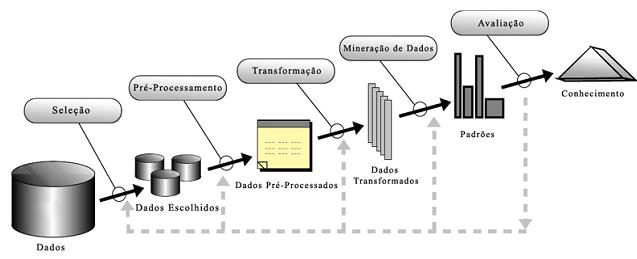
\includegraphics[scale=.65]{../img/kdd/pt.png}
	\caption{Ilustração das etapas da extração de conhecimento}
	\label{img:kdd}
\end{figure}

\begin{enumerate}
	\item \underline{Dados:}
	      conjunto de dados organizados de forma \textit{qualitativa} ou \textit{quantitativa} sobre determinado tema, no qual possibilidade a extração de informação que pode resultar em conhecimento.
	\item \underline{Pré-processamento dos dados:}
	      Selecionar os dados de acordo com a demanda do estudo, descartando assim dados irrelevantes, a fim de tornar a análise dos eficiente e eficaz.
	      As etapas são distribuídas:
	      \begin{itemize}
		      \item \underline{limpeza:} remoção de ruídos de dados inconsistentes e ausentes;
		      \item \underline{integração:}combinação dos dados de diferentes fontes;
		      \item \underline{seleção:} escolha de dados relevantes à análise; e
		      \item \underline{transformação:} consolidação dos dados em formato apropriado.
	      \end{itemize}
	\item \underline{Mineração de dados:}
	      Utilização de métricas e medidas estatísticas, para representar o conjunto de dados e a sua distribuição.
	      Tais medidas são análise descritiva, agrupamento, predição, associação e detecção de anomalias.
	\item underline{Avaliação:}
	      Identificar os padrões obtidos pela representação do conhecimento são válidos, ou seja, representativo.
\end{enumerate}


\subsection{Ferramentas}

\begin{itemize}
	\item Weka~(www.cs.waikato.ac.nz/ml/weka)
	\item Matlab
	\item R Studio~(www.r-project.org)
	      \begin{itemize}
		      \item Bioconductor~(www.bioconductor.org)
	      \end{itemize}
	\item Wolfram Mathematica~(www.wolfram.com/mathematica)
	\item RapidMiner~(rapidminer.com)
	\item SAS~(sas.com)
	\item SSPS by IBM~(www-01.ibm.com/software/analytics/spss)
	\item Orange~(orange.biolab.si)
	\item Mahout by Apache~(mahout.apache.org)
	\item ELKI~(elki.dbs.ifi.lmu.de): aprendizagem não supervisionado
	\item LIBSVM~(www.csie.ntu.edu.tw/~cjlin/libsvm)
\end{itemize}


\subsubsection*{Visualização de dados}
\begin{itemize} 
	\item \underline{Tableau:} visualização dinâmica dos dados e dashboard personalizado
	\item \underline{PowerBI:} integração com os serviços Microsoft
	\item \underline{Data Studio:} integração com os serviços Google
	\item \underline{Qlik:} licitação 
\end{itemize}


\subsubsection*{SGBD}
\begin{itemize}
	\item PostgreSQL~\footnote{www.postgresql.org}
	\item ORACLE~\footnote{www.oracle.com}
	\item SQL Server~\footnote{www.microsoft.com/en-us/server-cloud/products/sql-server}
	\item DB2~\footnote{www-01.ibm.com/software/data/db2}
\end{itemize}
	

\subsubsection*{Apache}
\underline{Airflow}~\footnote{https://airflow.apache.org/}: plataforma de gerenciamento de fluxo de trabalho de código aberto


\subsubsection*{Integração dos dados}
\begin{itemize}	
	\item Kafka\footnote{https://kafka.apache.org/}
	\item Spark\footnote{https://spark.apache.org/}
	\item NiFi\footnote{https://nifi.apache.org/}
\end{itemize}


\subsubsection*{Microsserviços}
\begin{itemize}	
	\item Docker
	\item Docker Compose
	\item Kubernet
\end{itemize}


\subsection{Material complementar}

Livros:
\begin{itemize}
	\item Introdução a mineração de dados por~\citeonline{mineracao_de_dados_br}
	\item Data Science para Negócios por~\citeonline{data_science_para_negocios}
	\item Python para análise de dados por~\citeonline{mckinney_pandas}
	\item Introdução à Ciência de Dados Fundamentos e Aplicações~\footnote{https://www.ime.usp.br/~jmsinger/MAE5755/cdados2019ago06.pdf}
\end{itemize}


Cursos:
\begin{itemize}
	\item ML4all - UFPR~\footnote{http://cursos.leg.ufpr.br/ML4all/1parte/}
\end{itemize}


Blog:
\begin{itemize}
	\item DIKW by Towards Data Science~\footnote{https://towardsdatascience.com/rootstrap-dikw-model-32cef9ae6dfb}
	\item Curso R~\footnote{https://blog.curso-r.com/}
	\item Tests as linear by Lindeloev~\footnote{https://lindeloev.github.io/tests-as-linear/}
	\item JTemporal~\footnote{https://jtemporal.com/}
\end{itemize}


Base de dados:
\begin{itemize}
	\item UCI Machine Learning Repository~\footnote{http://archive.ics.uci.edu/ml/index.php}
	\item KDnuggets~\footnote{https://www.kdnuggets.com/datasets/index.html}
	\item Governo Brasileiro~\footnote{https://dados.gov.br/}
	      \begin{itemize}
		      \item Brasil IO~\footnote{https://brasil.io/}
		      \item Gasto de parlamentar~\footnote{https://serenata.ai/}
	      \end{itemize}
	\item Governo Americano~\footnote{https://www.data.gov/}
	\item Governo do Inglês~\footnote{https://data.gov.uk/}
	\item PyData Book~\footnote{https://github.com/wesm/pydata-book}
\end{itemize}
